\documentclass{article}
\usepackage{amsmath}
\usepackage{mathtools}
\usepackage{gensymb}
\usepackage[a4paper,inner=1.5cm,outer=1.5cm,top=2cm,bottom=0.5cm]{geometry} 
\usepackage{xcolor}                    
\usepackage{tikz}                           
\usepackage{multicol}
\usepackage{pgfplots}
\usetikzlibrary{calc}
\usetikzlibrary{intersections}
\usetikzlibrary{intersections,calc,angles,quotes}
\usetikzlibrary{shapes,arrows,positioning,decorations.pathreplacing,calc}
\usetikzlibrary{calc,angles,positioning,intersections,quotes,decorations.markings}
\usepackage{tkz-euclide}
\usetikzlibrary{backgrounds}
\usetikzlibrary{calc,through}
\usetikzlibrary{angles}
\usetikzlibrary{fadings}
\usetikzlibrary{shapes.geometric}
\usetikzlibrary{shapes.symbols}
\usepackage{draftwatermark}
\usepackage{mathptmx}

\SetWatermarkText{\textcolor{black!30}{Mathema Shukur}}
\SetWatermarkFontSize{2 cm}
\usepackage[utf8]{inputenc}
\usepackage{fontspec}

\setmainfont{[Kalpurush.ttf]}
\newfontface{\en}{[Arial.ttf]} %%this is optional, if you want to use a secondary font. Any english font is supported
\newlength\Radius
\setlength\Radius{4cm}
\begin{document} 
	\Large
	\textcolor{red}{Welcome To} 
	\\
	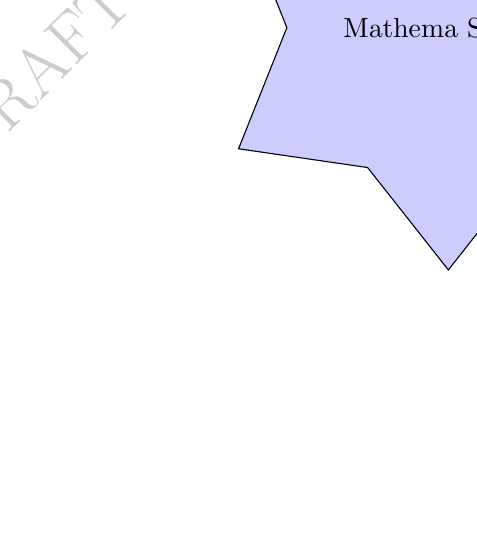
\begin{tikzpicture}
		\tikz \node [fill=blue!20,star,star points=6,draw] {Mathema Shukur };
	\end{tikzpicture}
	\\
	যাদের জন্যে প্রযোজ্যঃ  	\textcolor{magenta}{একাদশ ও দ্বাদশ শ্রেণীর শিক্ষার্থী} \\
	বিষয়ঃ \textcolor{magenta}{উচ্চতর গণিত ১ম পত্র} \\
	অধ্যায়ঃ \textcolor{magenta}{৩-সরলরেখা}\\ 
	Subtopicঃ  \textcolor{magenta}{  সরলরেখার বিভিন্ন আকারের সমীকরণ নির্ণয় করা   }\\
	\\
	\textcolor{blue}{(1)	ঢাল বিন্দু আকার Point slope form}\\
	\\
	$(y-y_1)=m(x-x_1)$\\
	\\
	\textcolor{red} {(2)  দুই বিন্দু আকার 	Two point form}\\
	\\
	$y-y_1=\left(\frac{y_1-y_2}{x_1-x_2}\right)(x-x_1)$\\
	\\
	\textcolor{green}{ (3) ঢাল খণ্ডন আকার 	Slope intercept form}\\
	\\
	$y=mx+c$\\
	\\
	\textcolor{cyan}{ (4) দ্বি খণ্ডন আকার  Two	Intercept form}\\
	\\
	$\frac{x}{a}+\frac{y}{b}=1$\\
	\\
		\\
	\textcolor{purple}{ (5) লম্ব  আকার  Normal form}\\
	\\
	মূল বিন্দু হতে কোনো সরলরেখার উপর অঙ্কিত লম্বের দৈর্ঘ্য $p$ এবং লম্বটি $x-$ অক্ষের ধনাত্মক দিকের সাথে $\alpha$ কোণ উৎপন্ন করলে, রেখাটির সমীকরণ নির্ণয় কর \\ 
	\\
	$x\cos \alpha +y\sin \alpha=p$\\
	\\
	\begin{multicols}{2}
	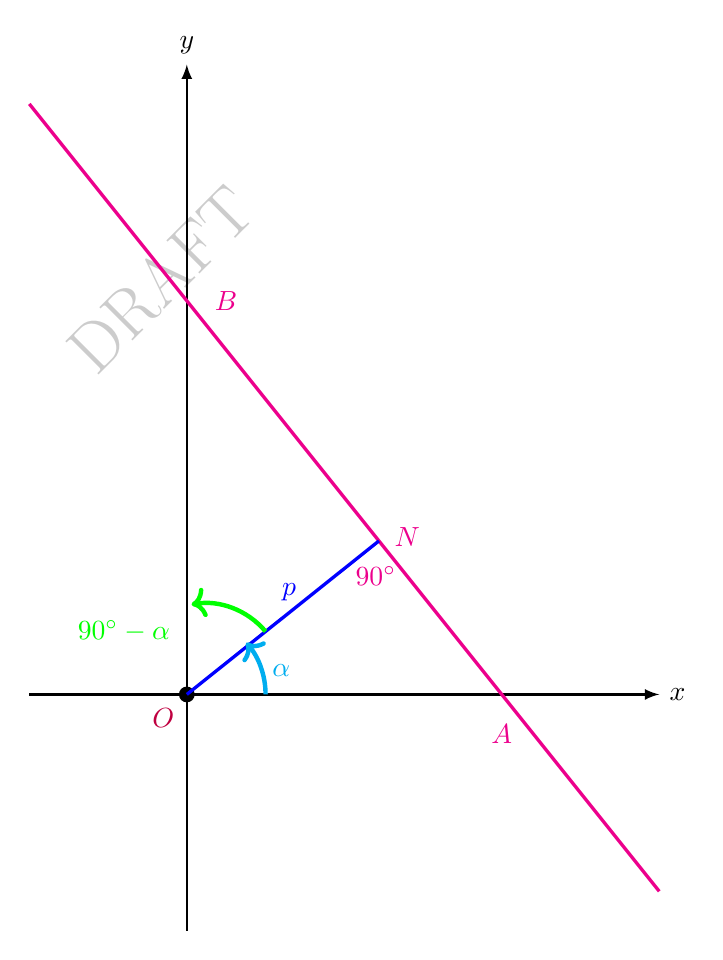
\begin{tikzpicture}[transform shape,scale=1]
		\draw [-latex,thick](-2,0) -- (6,0) node[right] {$x$} coordinate(x axis);
		\draw [-latex,thick](0,-3) -- (0,8) node[above] {$y$} coordinate(y axis);
		\fill[black] (0,0) circle (1 mm);
		\node at (-0.3,-0.3) {$\textcolor{purple}{O}$};	
		\node at (0.5,5) {$\textcolor{magenta}{B}$};	
		\node at (1.3,1.3) {$\textcolor{blue}{p}$};	
		\node at (4,-0.5) {$\textcolor{magenta}{A}$};	
		\node at (2.8,2) {$\textcolor{magenta}{N}$};	
		\node at (1.2,0.3) {$\textcolor{cyan}{\alpha}$};
		\node at (-0.8,0.8) {$\textcolor{green}{90\degree-\alpha}$};
		\node at (2.4,1.5) {$\textcolor{magenta}{90\degree}$};		
		\draw[very thick,magenta] (-2,7.5)--(6,-2.5);	
		\draw[very thick,blue] (0,0)--(2.44,1.95);	
		\draw[color=cyan,ultra thick, ->] (1,0) arc (0:41:1cm);	
		\draw[color=green,ultra thick, ->] (1,0.8) arc (40:100:1cm);	
	\end{tikzpicture}
	\\ 
	\begin{align*}
		\cos \alpha &=\frac{ON}{OA}\\
		\\
		\sec \alpha &=\frac{OA}{ON}\\
		\\
		OA&=ON\,\, \sec \alpha \\
		\\
		OA&=p\,\,\sec \alpha 
	\end{align*}
	\end{multicols}
\begin{multicols}{2}
	\begin{align*}
	\cos \left(90\degree-\alpha \right) &=\frac{ON}{OB}\\
	\\
	\sin \alpha &=\frac{ON}{OB}\\
	\\
	\mathrm{cosec} \alpha  &=\frac{OB}{ON}\\
	\\
	OB&=ON\,\, \mathrm{cosec} \alpha \\
	\\
	OB&=p\,\, \mathrm{cosec} \alpha \\
\end{align*}
\\
দ্বি খন্ডন আকার সমীকরণ  (Two intercept form)\\
\begin{align*}
	\frac{x}{OA}+\frac{y}{OB}&=1\\
	\\
	\frac{x}{p\,\,\sec \alpha }+\frac{y}{p\,\, \mathrm{cosec} \alpha}&=1\\
	\\
	\frac{x\,\,\cos \alpha}{p}+\frac{y\,\,\sin \alpha}{p}&=1\\
	\\
	x\,\,\cos \alpha+y\,\,\sin \alpha&=p
\end{align*}
\end{multicols}
\vspace{5cm}
	সিলেট বোর্ড-২০২১\\ 
		নিচের চিত্র হতে $AB$ রেখার সমীকরণ নির্ণয় কর \\ 
	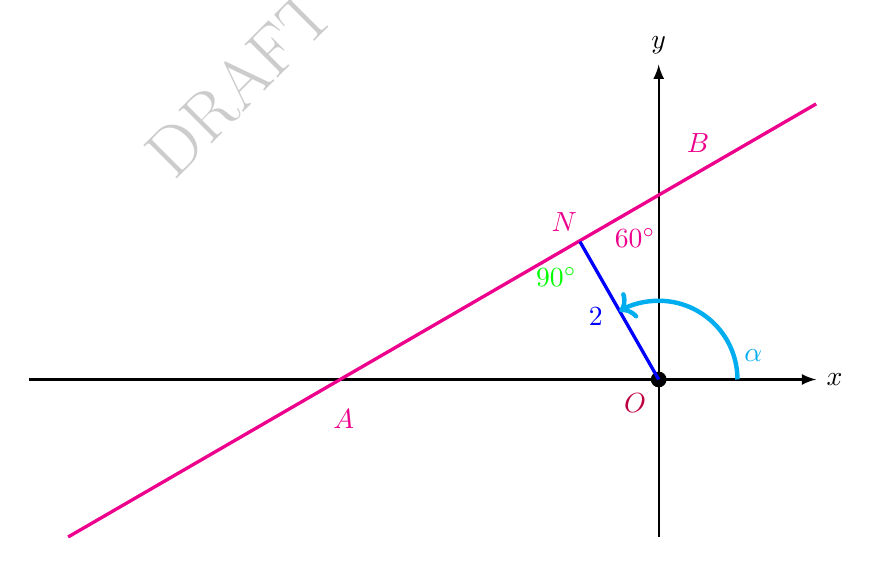
\begin{tikzpicture}[transform shape,scale=1]
		\draw [-latex,thick](-8,0) -- (2,0) node[right] {$x$} coordinate(x axis);
		\draw [-latex,thick](0,-2) -- (0,4) node[above] {$y$} coordinate(y axis);
		\fill[black] (0,0) circle (1 mm);
		\node at (-0.3,-0.3) {$\textcolor{purple}{O}$};	
		\node at (0.5,3) {$\textcolor{magenta}{B}$};	
		\node at (-0.8,0.8) {$\textcolor{blue}{2}$};	
		\node at (-4,-0.5) {$\textcolor{magenta}{A}$};	
		\node at (-0.3,1.8) {$\textcolor{magenta}{60\degree}$};	
		\node at (1.2,0.3) {$\textcolor{cyan}{\alpha}$};
		\node at (-1.3,1.3) {$\textcolor{green}{90\degree}$};
			\node at (-1.2,2) {$\textcolor{magenta}{N}$};
		\draw[very thick,magenta] (-7.5,-2)--(2,3.5);	
		\draw[very thick,blue] (0,0)--(-1,1.75);	
		\draw[color=cyan,ultra thick, ->] (1,0) arc (0:120:1cm);	
	\end{tikzpicture}
	\\ 
	মূল বিন্দু হতে $AB$ রেখার উপর অঙ্কিত লম্বের দৈর্ঘ্য $ON=2$ \\
	\\
	$ON$ লম্বটি $x-$ অক্ষের ধনাত্মক দিকের সাথে $\alpha$ কোণ তৈরী করে \\ 
	\\
	$\angle OBN=60\degree$,\qquad $\angle BON=30\degree $\\ 
	\\
	$\alpha=90\degree+30\degree=120\degree$\\ 
	\\
	লম্ব আকার সমীকরণ (Normal form)\\
	\begin{align*}
		x\,\, \cos \alpha +y\,\,\sin \alpha &=p\\
		\\
		x\,\,\cos 120\degree +y\,\,\sin 120\degree&=2\\
		\\
		x\,\, \left(-\frac{1}{2}\right)+y\,\, \frac{\sqrt{3}}{2}&=2\\
		\\
		-x+\sqrt{3}y&=4\\
		\\
		x-\sqrt{3}y+4&=0
	\end{align*}
\end{document}